\scanpage{107}
% archive sheet number: 106
\figure{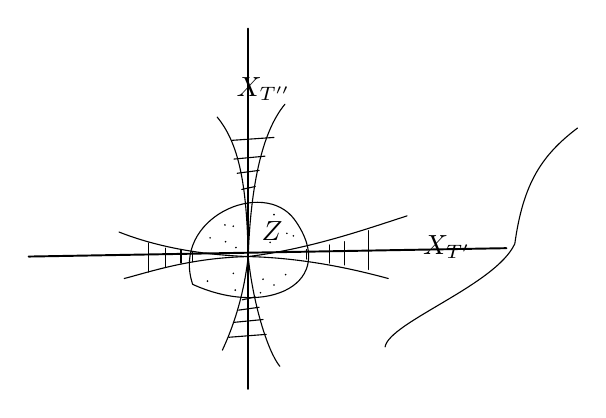
\begin{tikzpicture}[x=.82cm,y=.82cm,line cap=round]
\draw[line width=.7pt] (-3.40,0)--(4.00,.13);
\draw[line width=.7pt] (0,-2.05)--(0,3.53);
\draw (0,0) .. controls (-.02,1.14) and (-.15,1.76) .. (-.48,2.16);
\draw (0,0) .. controls (.04,1.12) and (.22,1.94) .. (.57,2.36);
\draw (0,0) .. controls (-.07,-.64) and (-.25,-1.13) .. (-.40,-1.45);
\draw (0,0) .. controls (.07,-.69) and (.29,-1.45) .. (.49,-1.70);
\draw (0,0) .. controls (-.80,.03) and (-1.47,.17) .. (-2.00,.38);
\draw (0,0) .. controls (-.90,-.02) and (-1.53,-.24) .. (-1.92,-.34);
\draw (0,0) .. controls (.96,.12) and (1.81,.42) .. (2.46,.63);
\draw (0,0) .. controls (.85,-.02) and (1.62,-.19) .. (2.17,-.34);
\draw (-.86,-.43) .. controls (-1.20,.60) and (.24,1.23) .. (.72,.57)
 .. controls (1.42,-.41) and (.30,-.96) .. (-.86,-.43);
\foreach \x/\a/\b in {-1.54/-.24/.21,-1.28/-.17/.13,-1.04/-.10/.10,-.86/-.08/.07,.91/-.04/.11,1.26/-.10/.18,1.49/-.13/.23,1.86/-.20/.40}
{\draw (\x,\a)--(\x,\b);}
\foreach \y/\a/\b in {1.80/-.25/.40,1.51/-.22/.26,1.29/-.17/.17,1.04/-.10/.11,-.67/-.09/.11,-.83/-.15/.17,-1.02/-.23/.23,-1.25/-.30/.28}
{\draw (\a,\y)--(\b,\y+.045);}
\foreach \x/\y in {-.59/.29,-.36/.49,-.23/.47,-.35/.23,-.19/.14,.40/.65,.60/.36,.70/.32,.34/.22,-.63/-.38,-.23/-.26,-.20/-.52,.23/-.35,.40/-.44,.58/-.28,.19/-.56}{\fill (\x,\y) circle (.014);}
\draw[thin] (2.12,-1.40) .. controls (2.18,-1.02) and (3.84,-.44) .. (4.13,.20) .. controls (4.26,1.15) and (4.56,1.58) .. (5.10,1.99);
\node at (.37,.39){$Z$};\node at (.24,2.60){$X_{T''}$};\node at (3.08,.15){$X_{T'}$};
\end{tikzpicture}}

\diagram{\begin{tikzcd}[ampersand replacement=\&,column sep=small,row sep=small]
\& \& \& \deleted{\unsure{*}} \& {}\\
\& \widehat{\mathbb Z}=\pi_1(Z')\arrow[dl]\arrow[drrr] \& \& \pi_1(Z'')=\widetilde{\mathbb Z}\arrow[dl]\arrow[dr] \& {}\\
\pi_1(X_{T'})\arrow[drr] \& \& \pi_1(X_{T''})\arrow[d] \& \& \pi_1(Z)=\widehat{\mathbb Z}^{\,2}\arrow[dll]\\
\& \& \pi_1(X_T) \& \& {}
\end{tikzcd}}

$Z=\operatorname{Spec}\widehat{\underline{\mathrm O}_{X,a}}$\inserted{$A$}

$X_{T'}\cap X_{T''}=\varnothing$

$X_{T'}\cap Z_{\deleted{\unsure{T'}}}=Z'=\widehat A_{p'}$ correspond au corps
résiduel $k(p')={}$ corps local en $a$ de $T'_0$

$X_{T''}\cap Z=Z''=\widehat A_{p''}$ correspond au corps
résiduel $k(p'')={}$ corps local en $a$ de $T''_0$

On doit prouver un \uline{\unsure{th|thm|th.} de descente}
de nature essentiellement locale

$+$ déterminer certains hom. canoniques

\[
-\quad-\quad-
\]

\diagram{\begin{tikzcd}[ampersand replacement=\&,row sep=tiny]
\deleted{\unsure{A'}}\arrow[d,no head,bend right=12]\\ A\arrow[d]\\ B
\end{tikzcd}}
